\documentclass[11pt]{article}
\usepackage{amsmath,amssymb,amsthm}
\usepackage{enumitem}
\usepackage[left=1in,right=1in,top=1in,bottom=1in]{geometry}
\usepackage{tikz}
\usetikzlibrary{cd,decorations.pathmorphing}
\usepackage{xcolor}
\usepackage{sectsty,wrapfig}
\usepackage{hyperref}


\newtheorem{thm}{Theorem}[section]
\newtheorem{prp}[thm]{Proposition}
\newtheorem{lmm}[thm]{Lemma}
\newtheorem{crl}[thm]{Corollary}
\newtheorem{ques}[thm]{Question}
\newtheorem{fact}[thm]{Fact}

\theoremstyle{definition}
\newtheorem{dfn}[thm]{Definition}
\newtheorem{eg}[thm]{Example}

\theoremstyle{remark}
\newtheorem{rmk}[thm]{Remark}

\def\wt#1{\widetilde{#1}}
\def\ov#1{\overline{#1}}
\def\mr#1{{\mathring{#1}}}


\def\Z{\mathbb{Z}}
\def\C{\mathbb{C}}
\def\P{\mathbb{P}}
\def\R{\mathbb{R}}
\def\Q{\mathbb{Q}}
\def\D{\mathbb{D}}
\def\M{\mathfrak{M}}
\def\cA{\mathcal{A}}
\def\cD{\mathcal{D}}
\def\cG{\mathcal{G}}
\def\cM{\mathcal{M}}
\def\cT{\mathcal{T}}
\def\cN{\mathcal{N}}
\def\rI{{\mathring{I}}}

\def\cmt#1{\textcolor{purple}{(#1)}}
\def\tn#1{\textnormal{#1}}
\def\pr{{\textnormal{pr}}}


\begin{document}

\setlength{\parskip}{\baselineskip}
\setlength{\parindent}{0cm}

\section{Introduction}

.....(introduction)

{\bf Define the kind of bundle we work with in this paper:}
Given a smooth homology sphere $M$, define a {\it framed $(M,\infty)$-bundle} $(\pi:E\to B,\sigma, \tau, F)$ (abbreviate all these to $\pi$) to be a smooth fiber bundle $\pi:E\to B$ with fiber $M$, with a smooth section $\sigma$, a trivialization $\tau$ of the bundle near $\sigma$, and a smooth vertical framing $F$ of $\pi$ ``standard'' near $\sigma$. 

{\bf Define the bracket operation, $\pi_1,\pi_2\to[\pi_1,\pi_2]$ on such bundles, in an intuitively clear but not necessarily rigorous way.}

{\bf Define cobracket and coproduct on graph cohomology (everything is over $\Q$):}
\begin{itemize}
\item First, define the graph complex $\cG'$---the $\Q$-vector space spanned by (with correct orientation definition, omitted here) connected graphs containing either a univalent vertex or a simple loop (an edge starting and ending at the same vertex). 
The coboundary operation $\delta$ is given by contracting an edge. 
In $\delta$ and all the operations on graphs below, whenever a graph not in $\cG'$ appears (a graph that has a univalent vertex or simple loop), we set it to 0. 
\item Taking the homology of $\cG'$ with respect to $\delta$, denote by $H^*{\cG'}$. 

\item Define the cobracket operation to be the linear map
\begin{align*}
\Delta_{[,]}: \cG'&\longrightarrow\cG'\otimes\cG'\\
\Gamma&\longrightarrow \sum_{\Gamma'\le\Gamma}\big(\Gamma'\otimes\Gamma/\Gamma'+(-1)^{..}\Gamma/\Gamma'\otimes\Gamma'\big), 
\end{align*}
where $\Gamma'$ ranges through all full subgraphs of $\Gamma$ that is connected, with no univalent vertex or simple loop.
\item Check that $\Delta_{[,]}$ commutes with $\delta$ and $\delta\otimes\tn{id}\pm\tn{id}\otimes\delta$, so it descends to 
$$\Delta_{[,]}: H^*{\cG'}\longrightarrow H^*(\cG'\otimes\cG')\approx H^*{\cG'}\otimes H^*{\cG'}.$$

\item Finally we also define the coproduct operation on $\cG'$ (this makes more sense for disconnected graphs but w=for connected graphs it is extra simple):  
\begin{align*}
\Delta_{\cdot}: \cG'&\longrightarrow \cG'\otimes\cG'\\
\Gamma&\longrightarrow \Gamma\otimes \tn{(the empty graph)} + \tn{(the empty graph)}\otimes\Gamma.
\end{align*}

\end{itemize}

{\bf Brief introduction to Kontsevich's characteristic classes.}
Given a framed $(M,\infty)$-bundle $\pi:E\to B$ as above, denote by  
$$K_\pi: H^*(\cG')\longrightarrow H^*(B)$$
Kontsevich's characteristic classes of $\pi$. 


\begin{thm}\label{formula_thm}
Suppose $d\ge3$. 
For $i=1,2$, suppose $M_i$ is a $d$-dimensional smooth homology sphere and 
suppose $\pi_i: E_i\to B_i$ is a framed $(M,\infty)$-bundle. 
(Now, $[\pi_1,\pi_2]: E\to S^d\times B_1\times B_2$ is the bracket bundle.)
Then, for all $\eta\in H^*\cG'$, 
\begin{align*}
K_{[\pi_1,\pi_2]}(\eta)=
\tn{PD}_{S^d}[S^d]\otimes
(K_{\pi_1}\otimes K_{\pi_2})(\Delta_{[,]}(\eta))
+\tn{PD}_{S^d}[pt]\otimes
(K_{\pi_1}\otimes K_{\pi_2})(\Delta_\cdot(\eta)).
\end{align*}
(Both LHS and RHS lives in 
$$H^*(S^d\times B_1\times B_2)\approx H^*(S^d)\otimes H^*(B_1)\otimes H^*(B_2).$$
$\tn{PD}_{S^d}$ means Poincar\'e dual on $S^d$; $[S^d]$ stands for the fundamental class of $S^d$ and $[pt]$ stands for the point class of $S^d$.)
\end{thm}


......(Then talk about the $(d+1)$-fold loop space structure on $\tn{BDiff}^{\tn{fr}}_\partial(D^d)$ and the theorem/corollary that it doesn't extend.)

(Below is an outline of the proof of Theorem \ref{formula_thm}.
Throughout, $\pi_1,\pi_2$ are given and fixed. 
)

\section{Conftilde}\label{conftilde_sec}

Construct the big configuration space $\widetilde{C}_n$. 
Show that it is a smooth manifold with boundary and corners. 
(These are mostly already written in the file ``conftilde'' I sent a while ago.)

Here is a schematic picture of $\wt{C}_n$ (the marked points are not drawn; the actual stratification structure of $\wt{C}_n$ is more complicated than what is shown in the picture): 

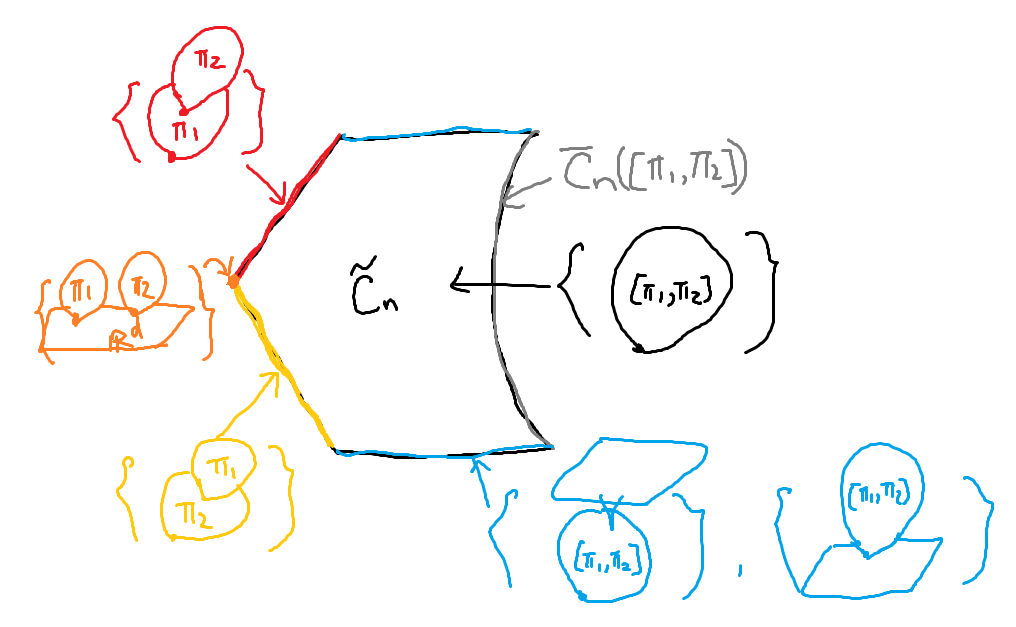
\includegraphics[scale=0.7]{conftilde.png}

The boundary of $\wt{C}_n$ consists of 3 parts: 
\begin{itemize}
\item the gray part is $\ov{C}_n([\pi_1,\pi_2])$;
\item the blue part is a 1-parameter family of $\partial \ov{C}_n([\pi_1,\pi_2])$---its interior is diffeomorphic to 
$$\partial \ov{C}_n([\pi_1,\pi_2])\times (0,1);$$
\item $\ov{C}^*_n$, consisting of the red, orange, and yellow parts. 
\end{itemize}

\section{Propagators}

Fix a volume form $\omega_0$ on $S^{d-1}$. 
For $i=1,2$, fix a propagator $\omega_i$ on $\ov{C}_2(\pi_i)$ such that on $\partial\ov{C}_2(\pi_i)$, $\omega_i$ is given by $\omega_0$. 

\subsection{Propagator on confstar}

$\omega_1,\omega_2$ naturally induce a propagator $\omega_*$ on $\ov{C}^*_2$. On the main strata of $\ov{C}^*_2$, define $\omega_*$ as follows: 
\begin{itemize}
\item On the stratum $S_{11}$ consisting of  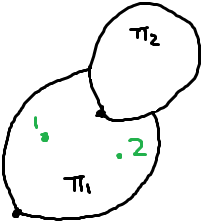
\includegraphics[scale=0.4]{mouse11}, 
there is the forgetful map
$f_{11}:S_{11}\to \ov{C}_2(\pi_1)$. We define $\omega_*|_{S_{11}}=f_{11}^*(\omega_1)$. 

\item On the stratum $S_{22}$ consisting of  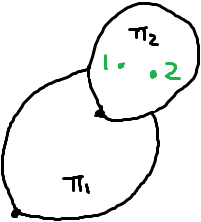
\includegraphics[scale=0.4]{mouse22}, 
there is the forgetful map
$f_{22}:S_{22}\to \ov{C}_2(\pi_2)$. We define $\omega_*|_{S_{22}}=f_{22}^*(\omega_2)$. 

\item On the stratum $S_{12}$ consisting of  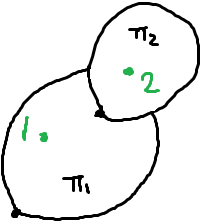
\includegraphics[scale=0.4]{mouse12}, 
there is the forgetful map
$f_{12}:S_{12}\to \ov{C}_2(\pi_1)$, where the second marked point is considered to be located at the node on $\pi_1$.  
We define $\omega_*|_{S_{22}}=f_{22}^*(\omega_2)$.

\item ...(There are 5 more situations, all variations of the above, permuting $\pi_1,\pi_2, 1,2$.) 
\end{itemize}

We then check that the above definitions are compatible when the main strata glue together. 
For example, the stratum $S'$ consisting of 
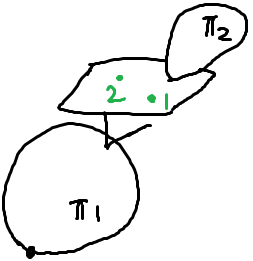
\includegraphics[scale=0.4]{S11capS22} lies in the intersection of $\ov{S}_{11}$ and $\ov{S}_{22}$;
but the $\omega_*$ constructed on $S_{11}$ and on $S_{22}$, when extended to here, agree, 
since they both become $(f')^*\omega_0$, where $f':S'\to S^{d-1}$ is the forgetful map recording the direction of the vector between the two points.

All other codimension-1 strata can be straight-forwardly checked like this as well. 
We may need to check higher-codimension strata as well but it shouldn't be hard.

\begin{rmk}
I lied a bit---``compatibility'' of $\omega_*$ along the gluing is a stronger condition then it is presented above. 
Given two manifolds with boundary, $X,Y$, such that $\partial X\approx \partial Y=:W$, let $Z$ be the space obtained by gluing $X,Y$ together along their common boundary $W$, but we do not specify a smooth structure near $W$;
then, say a form $\alpha$ on $X$ is compatible with a form $\beta$ on $Y$ if 
\begin{itemize}
\item $\alpha|_W=\beta|_{W}$;
\item there are collar neighborhoods $N_X$ of $W$ in $X$ and $N_Y$ of $W$ in $Y$ (with projection maps $p_X:N_X\to W$, $p_Y:N_Y\to W$) such that 
$\alpha|_{N_X}=p_X^*\alpha|_W$, $\beta|_{N_Y}=p_Y^*\beta|_W$. 
\end{itemize} 
The second condition says that in a collar neighborhood of the boundary the forms are trivial in the normal direction. 
In our situation, this stronger compatibility condition should be achievable as well, if we impose a similar condition (``parallel to boundary'' near the boundary) on $\omega_1,\omega_2$. 
\end{rmk} 

\subsection{Propagator on other parts of the boundary of conftilde}

To define a propagator on the blue part of $\partial\wt{C}_2$, we have no choice but to define it as induced from $\omega_0$ in the usual way. 

To define a propagator in the gray part of $\partial\wt{C}_2$, we just choose any propagator $\omega$ on $\wt{C}_2([\pi_1,\pi_2])$, so that $\omega|_{\partial\wt{C}_2([\pi_1,\pi_2])}$ is induced from $\omega_0$. 

Now we have defined a propagator on all of $\partial\wt{C}_2$. 

\subsection{Extend the propagator to the interior}

To show that there exists a closed form on $\wt{C}_2$ extending the propagator we just defined on $\partial\wt{C}_2$, 
it suffices to show that the map 
$$H^{d-1}(\wt{C}_2)\xrightarrow{\tn{restriction}}H^{d-1}(\partial\wt{C}_2)$$
is surjective. 
It is therefore sufficient to show that $H^d(\wt{C}_2,\partial\wt{C}_2)=0$. But 
\begin{align*}
H^*(\wt{C}_2,\partial\wt{C}_2)\approx
H_{\dim(\wt{C}_2)-*}(\wt{C}_2-\partial\wt{C}_2)=
H_{\dim(\wt{C}_2)-*}\big(C_2([\pi_1,\pi_2])\times (0,1)\big)\\
\approx
H_{\dim(\wt{C}_2)-*}({C}_2([\pi_1,\pi_2]))
\approx H^{*-1}\big(\ov{C}_2([\pi_1,\pi_2]),\partial\ov{C}_2([\pi_1,\pi_2])\big), 
\end{align*}
%$\dim(\wt{C}_2)=\dim(C_2([\pi_1,\pi_2]))+1=3d+1+\dim(B_1)+\dim(B_2)$ 
and this is 0 when $*-1<d+1$; see the proof of Lemma 2.12 in \href{https://arxiv.org/pdf/2109.01609}{Watanabe's addendum paper}. 

We choose and fix such an extension. This gives us a propagator $\wt\omega$ on $\wt{C}_2$. 

\section{Configuration space integrals}

For simplicity here we will only sketch part of the proof of Theorem \ref{formula_thm}, namely we only justify the first term on the RHS. 
(The second term is slightly more complicated but not much: basically because we only work with the point class on $S^d$---it is only 0-dimensional so you can still easily achieve transversality as needed. The second term is not needed for the corollary about the loop space structure on $\tn{BDiff}^{\tn{fr}}_\partial(D^d)$ either.) 

Given a graph $G$, we denote by $V(G)$ its vertex set and $E(G)$ its edge set. 

Suppose $\Gamma$ is a cocycle in graph cohomology. (For the simplicity of notation we assume $\Gamma$ is one graph---when it is a formal sum everything works as well.)

For every edge $e$ of $\Gamma$, we have the forgetful map 
$$f_e:\wt{C}_{V(\Gamma)}\longrightarrow\wt{C}_2.$$
And, when restricted to the gray (resp. red, orange, and yellow) part of $\partial\wt{C}_{V(\Gamma)}$, it is the forgetful map
$$f_e:\ov{C}_{V(\Gamma)}([\pi_1,\pi_2])\longrightarrow\ov{C}_2([\pi_1,\pi_2]) \qquad (\tn{resp. } f_e:\ov{C}^*_{V(\Gamma)}\longrightarrow\ov{C}^*_2).$$
Now we have the form $\bigwedge_{e\in E(\Gamma)}f_e^*\wt{\omega}$ on $\wt{C}_{V(\Gamma)}$. 
When restricted to the gray part of $\partial\wt{C}_n$, it is used to define Kontsevich's classes for the bundle $[\pi_1,\pi_2]$. 

To compute the ($\tn{PD}_{S^d}[S^d]$)-part of $K_{[\pi_1,\pi_2]}([\Gamma])$, we only need to compute, given arbitrary homology classes $\alpha_1\in H_*(B_1)$ and $\alpha_2\in H_*(B_2)$, the evaluation
$$\big\langle K_{[\pi_1,\pi_2]}([\Gamma]), [S^d]\otimes\alpha_1\otimes\alpha_2 \big\rangle.$$
For $i=1,2$, suppose $\alpha_i$ is represented by a sub-pseudo-manifold $\iota_i:B'_i\hookrightarrow B_i$. (For simplicity you can think of a smooth submanifold instead.)

For any $n$: notice that the projection map 
$\wt{p}:\wt{C}_n\to B_1\times B_2$
is a fiber bundle, and so is the restriction of $\wt{p}$ to each stratum of $\wt{C}_n$.
Let us pull everything back along $(\iota_1,\iota_2)$, so that the base gets changed to $B'_1\times B'_2$ instead of $B_1\times B_2$. 
Abusing notation, we still denote by
$\wt{C}_n,\ov{C}_n([\pi_1,\pi_2]),\ov{C}^*_n$
their pull-backs. 

Now, we have 
\begin{equation}
\label{integral_eqn}
\big\langle K_{[\pi_1,\pi_2]}([\Gamma]), [S^d]\otimes\alpha_1\otimes\alpha_2 \big\rangle=
\int_{\ov{C}_{V(\Gamma)}([\pi_1,\pi_2])}\bigwedge_{e}f_e^*{\omega}=
\int_{\tn{gray part of }\partial\wt{C}_{V(\Gamma)}}\bigwedge_{e}f_e^*\wt{\omega}.
\end{equation}
By Stocks' Formula (and the fact that $\wt\omega$ is closed), 
$$\int_{\partial\wt{C}_{V(\Gamma)}}\bigwedge_{e}f_e^*\wt{\omega}=\int_{\wt{C}_{V(\Gamma)}}d\Big(\bigwedge_{e}f_e^*\wt{\omega}\Big)=0,$$
so, 
$$(\ref{integral_eqn})=\int_{\tn{blue part of }\partial\wt{C}_{V(\Gamma)}}\bigwedge_{e}f_e^*\wt{\omega}+\int_{\ov{C}^*_{V(\Gamma)}}\bigwedge_{e}f_e^*{\omega_*}.$$
Since $\Gamma$ is a cocycle in graph cohomology, the first term is 0 just like in the proof of the well-definedness of Kontsevich's classes, so
$$\big\langle K_{[\pi_1,\pi_2]}([\Gamma]), [S^d]\otimes\alpha_1\otimes\alpha_2 \big\rangle=
\int_{\ov{C}^*_{V(\Gamma)}}\bigwedge_{e}f_e^*{\omega_*}.$$

\section{Configuration space integral on confstar}

We continue with the notation from last section (in particular, everything is over $B'_1, B'_2$ instead of $B_1, B_2$). 

It remains to show that 
\begin{equation}\label{stardecompose_eqn}
\big\langle (K_{\pi_1}\otimes K_{\pi_2})(\Delta_{[,]}[\Gamma]), \alpha_1\otimes\alpha_2 \big\rangle=
\int_{\ov{C}^*_{V(\Gamma)}}\bigwedge_{e}f_e^*{\omega_*}. 
\end{equation}
For a graph $G$, we denote by $V(G)$ its vertex set and $E(G)$ its edge set. 
The LHS above equals to\footnote{
A little more argument needed for this claim, but it is true.} 
\begin{align*}
\sum_{\Gamma'\le\Gamma}
\Big(&\int_{\ov{C}_{V(\Gamma')}(\pi_1)}
\bigwedge_{e\in E(\Gamma')}f_e^*\omega_1\Big)
\cdot
\Big(\int_{\ov{C}_{V(\Gamma/\Gamma')}(\pi_2)}
\bigwedge_{e\in E(\Gamma/\Gamma')}f_e^*\omega_2\Big)\\
&\pm
\Big(\int_{\ov{C}_{V(\Gamma/\Gamma')}(\pi_1)}
\bigwedge_{e\in E(\Gamma/\Gamma')}f_e^*\omega_1\Big)
\cdot
\Big(\int_{\ov{C}_{V(\Gamma')}(\pi_2)}
\bigwedge_{e\in E(\Gamma')}f_e^*\omega_2\Big).
\end{align*}
To prove (\ref{stardecompose_eqn}), it suffices to show that 
\begin{equation}\label{yellow_eqn}
\sum_{\Gamma'\le\Gamma}
\Big(\int_{\ov{C}_{V(\Gamma')}(\pi_1)}
\bigwedge_{e\in E(\Gamma')}f_e^*\omega_1\Big)
\cdot
\Big(\int_{\ov{C}_{V(\Gamma/\Gamma')}(\pi_2)}
\bigwedge_{e\in E(\Gamma/\Gamma')}f_e^*\omega_2\Big)=
\int_{\tn{yellow part of }\ov{C}^*_{V(\Gamma)}}\bigwedge_{e\in E(\Gamma)}f_e^*{\omega_*}
\end{equation}
and 
\begin{equation}\label{red_eqn}
\sum_{\Gamma'\le\Gamma}
\Big(\int_{\ov{C}_{V(\Gamma/\Gamma')}(\pi_1)}
\bigwedge_{e\in E(\Gamma/\Gamma')}f_e^*\omega_1\Big)
\cdot
\Big(\int_{\ov{C}_{V(\Gamma')}(\pi_2)}
\bigwedge_{e\in E(\Gamma')}f_e^*\omega_2\Big)=
\int_{\tn{red part of }\ov{C}^*_{V(\Gamma)}}\bigwedge_{e\in E(\Gamma)}f_e^*{\omega_*};
\end{equation}
here the ``red'' and ``yellow'' refers to the $\wt{C}_n$ picture in Section \ref{conftilde_sec}. 
Below we only prove (\ref{yellow_eqn}) since (\ref{red_eqn}) is completely similar. 

The yellow part of $\ov{C}^*_{V(\Gamma)}$ is simply
$$\sum_{V_1,V_2:V_1\sqcup V_2=V(\Gamma)}
\ov{C}_{V_1}(\pi_1)\times\ov{C}_{V_2\sqcup\{\star\}}(\pi_2),
$$
where $\star$ records the position of the node on $\pi_2$.
Therefore, the RHS of (\ref{yellow_eqn}) is
$$\sum_{V_1,V_2:V_1\sqcup V_2=V(\Gamma)}
\int_{\ov{C}_{V_2\sqcup\{\star\}}(\pi_2)}\int_{\ov{C}_{V_1}(\pi_1)}
\bigwedge_{\begin{subarray}{c}e\in E(\Gamma)\\\tn{both endpoints of }e\tn{ are in }V_1\end{subarray}}f_e^*{\omega_*}\wedge
\bigwedge_{\begin{subarray}{c}e\in E(\Gamma)\\ \exists\tn{ endpoint of }e\tn{ in }V_2\end{subarray}}f_e^*{\omega_*}. 
$$ 
For $V_1\subset V(\Gamma)$, we denote by $\Gamma'(V_1)$ the subgraph of $\Gamma$ spanned by vertices in $V_1$. Then, by the way $\omega_*$ is constructed, and by Fubini's Theorem, 
the above equals to 
$$\sum_{V_1,V_2:V_1\sqcup V_2=V(\Gamma)}
\Big(\int_{\ov{C}_{V_1}(\pi_1)}
\bigwedge_{e\in E(\Gamma'(V_1))} 
f_e^*{\omega_1}\Big)
\cdot
\Big(\int_{\ov{C}_{V_2\sqcup\{\star\}}(\pi_2)}
\bigwedge_{e\in E(\Gamma/\Gamma'(V_1))}
f_e^*{\omega_2}\Big). 
$$ 
This proves (\ref{yellow_eqn}). 


\end{document}